\section{Context}
% 1-2 pages max
Technologies have revolutionised the manufacturing industry ever since the Industrial revolution in the 19th century.
Robots are increasing productivity by replacing humans for arduous and repetitive manual tasks.
%are increasing productivity, efficiency, lower costs, and relieve humans from operationally dangerous tasks.
There is a noticeable increase in industrial robot order requests, as well as capital investments into the field.
Although robots can be superior in automating human tasks, there remain many that cannot be completely taken over and that still need human intervention, such as high-precision tasks.
To allow both human precision and robot automation, collaborative robots have been introduced.

\subsection{Cobotics}\label{subsec:Cobotics}
Collaborative robots, or \textit{cobots}, have been introduced by \cite{colgate1999cobots} and allow for a close collaboration between humans and robots.
They enable humans to perform tasks, which they cannot perform on their own, due to physical constraints such as the manipulation of heavy parts.
Furthermore, they reduce risks of work-related accidents, including health hazards such as exposure to dangerous environments (e.g. chemical acids, excessive temperatures or noise), as well as sleeping disorders caused by rotating work shifts.
Thus, cobots contribute to productivity gains as they are designed to take over manual and repetitive tasks and are able to respond to actions of the human operator.
While replacing jobs of low-skilled human workers, they open up a market for new high-skilled jobs.

Cobotic systems have been adopted in several industries from the food-processing industry (\cite{Food}), to aeronautics (\cite{Airbus}) to the health industry (\cite{Ebola}).
However, companies which resist the use of robots in their daily routines, consider the investment cost ineffective, due to their high initial costs and the lack of trained personnel.
%, who have the needed programming skills to fully operate and exploit the robots.
Traditional robot programming solutions require domain experts and robots are generally programmed to complete a specific task.
Recent approaches using large amounts of data (e.g. Neural Networks (\cite{billard2001robust})) or self-exploration (e.g. Reinforcement Learning (\cite{smart2002effective})) become infeasible for task-specific applications.
This is a bottleneck for industries as many robot programming solutions fail as the deployment in real world scenarios introduces further limitations. 
Thus, recent research has been focusing on robot programming for end-users.

\subsection{Robot Programming by Demonstration}
Robot Programming by Demonstration (PbD), also referred to as \textit{Learning from Demonstration}, is an end-user programming technique for teaching a robot new skills by demonstrating a task, without writing code (\cite{billard2008robot}).
Influenced by natural learning paradigms in humans and other animals, it is an intuitive robot programming method, with the goal to refine the robot's performance, by providing repetitive demonstrations.
PbD has become a central topic in research areas, with the aim to move from purely pre-programmed robots to flexible user-based interfaces for training robots.

Figure \ref{fig:Principle Overview} shows the life-cycle for teaching a robot by demonstration.
The teacher demonstrates the desired behaviour to the robot.
The robot uses its sensors for a multi-modal perception of the demonstration and extracts the relevant information to create a model of the skill.
The new skill is executed in a new context and evaluated by the teacher.
The teacher can refine the learned skill by providing additional demonstrations of the same skill.
The robot then generalises over the demonstrations by extracting relevant features that remained unchanged across the set of demonstrations.
This incremental learning process allows the robot to acquire a new skill from demonstrations provided by non-expert users.

\begin{figure}[h]
	\centering
	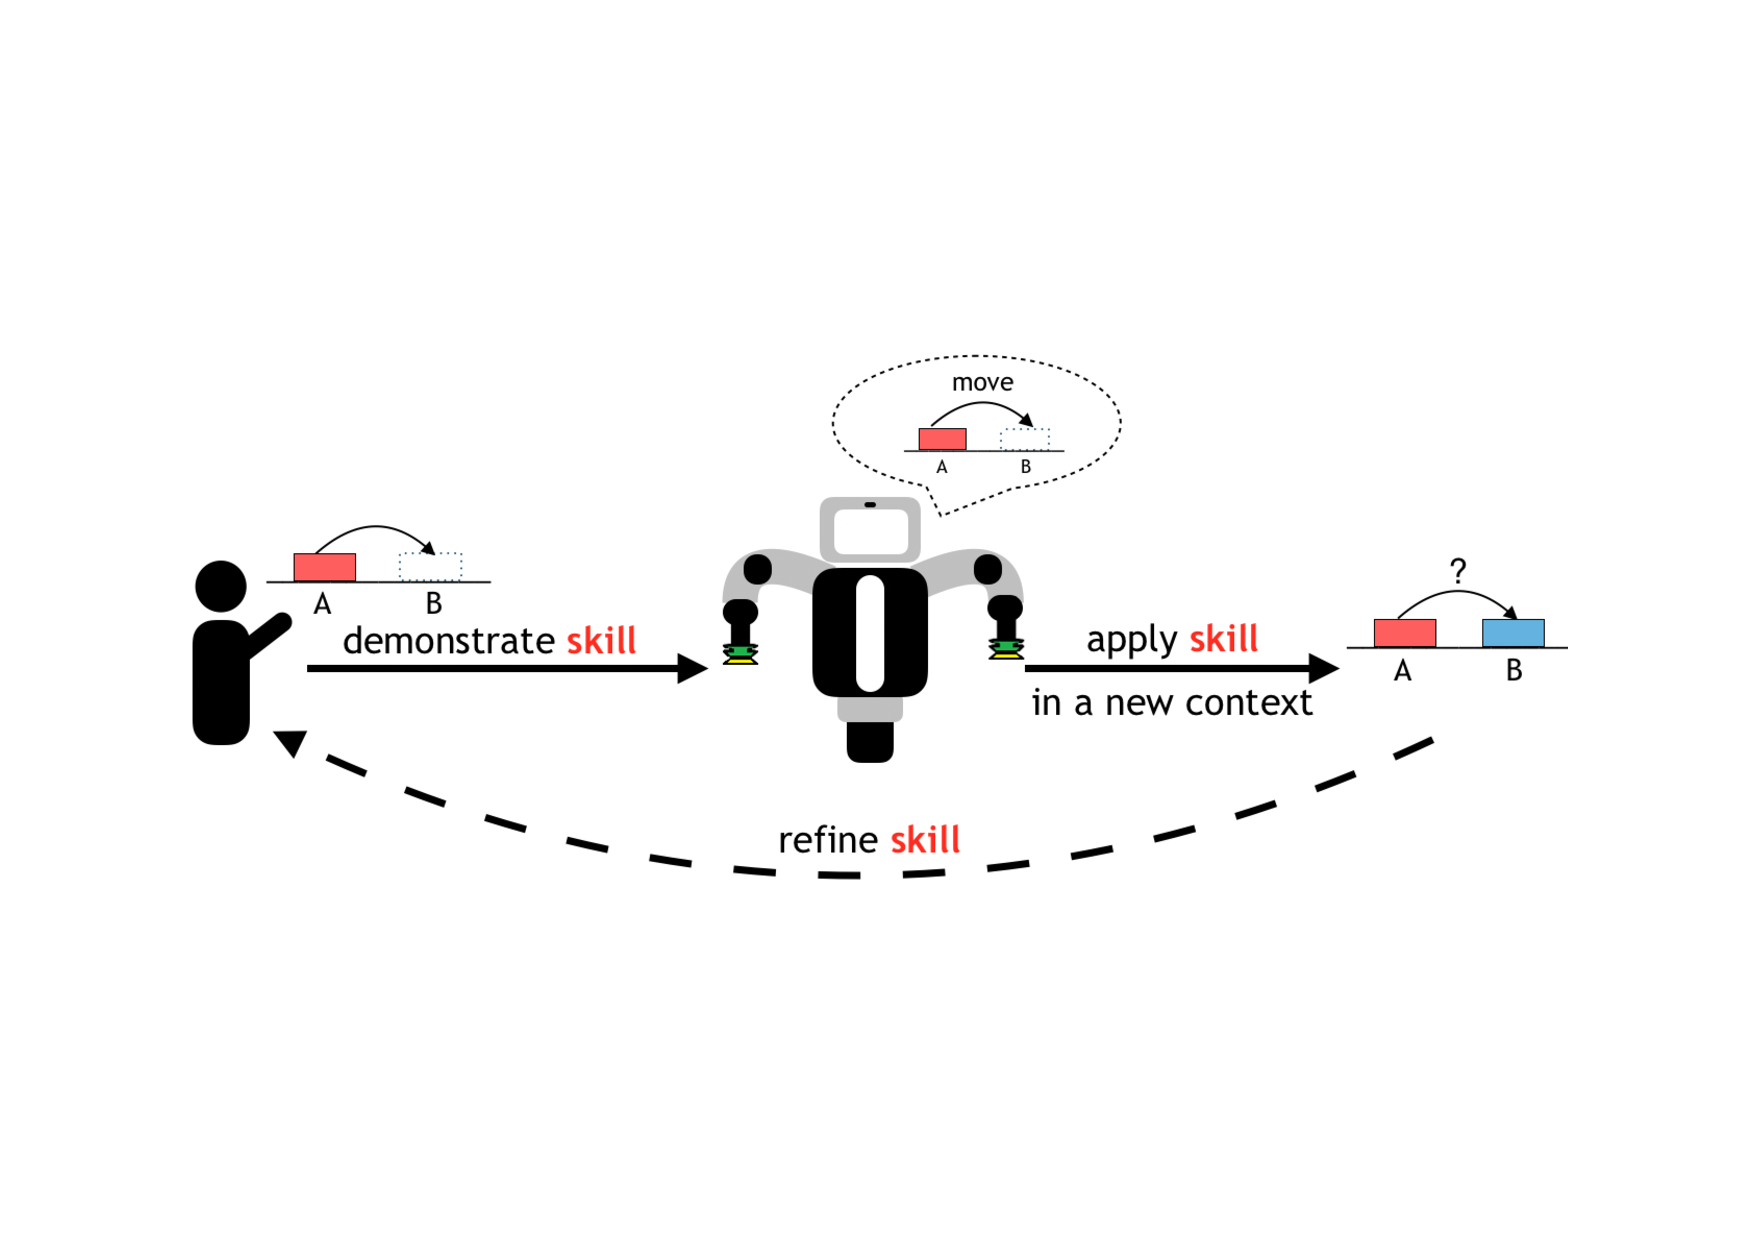
\includegraphics[width=0.5\linewidth]{figures/PbD-Overview}
	\caption{PbD Overview}
	\label{fig:Principle Overview}
\end{figure}

%Besides the advantage of being able to teach the robot tasks without the need to write code, PbD provides a powerful tool to improve learning abilities by reducing the search space of possible solutions.
However, learning object manipulation tasks is still considered a hard problem, as the robot has limited knowledge about the world and restricted sensor availability (\cite{ekvall2008robot}).
Many PbD algorithms have been proposed in the literature (\cite{argall2009survey,billing2010formalism}), but there still remain several challenges such as the suboptimality of demonstrations (\cite{chen2003programing,kaiser1995obtaining}) or the lack of comparative user studies (\cite{suay2012practical}).

% teaching full action sequences
Another major problem is that the robot is generally demonstrated an action sequence to complete a specific task (\cite{orendt2016robot,peppoloni2014ros}).
Take for example the Tower of Hanoi problem (\cite{douglas1985metamagical}) as shown in \fig{fig:Tower of Hanoi}a.
The objective is to move the entire stack to another rod, obeying the following simple rules:
\begin{itemize}
\item Only one disk can be moved at a time.
\item Each move consists of taking the upper disk from one of the stacks and placing it on top of another stack.
\item No disk may be placed on top of a smaller disk.
\end{itemize}

The robot can be taught an action sequence to solve the problem with three disks.
When the problem changes to four disks (\fig{fig:Tower of Hanoi}b), the robot has to be demonstrated a new sequence, even though both problems obey the same rules.
This is a complicated and time-consuming process and does not allow non-experts to reprogram robots for different tasks.
Ideally, we only teach the robot the objective and rules and let it generate the solution, or a \textit{plan}, on its own.

\begin{figure}[htp]
	\centering
	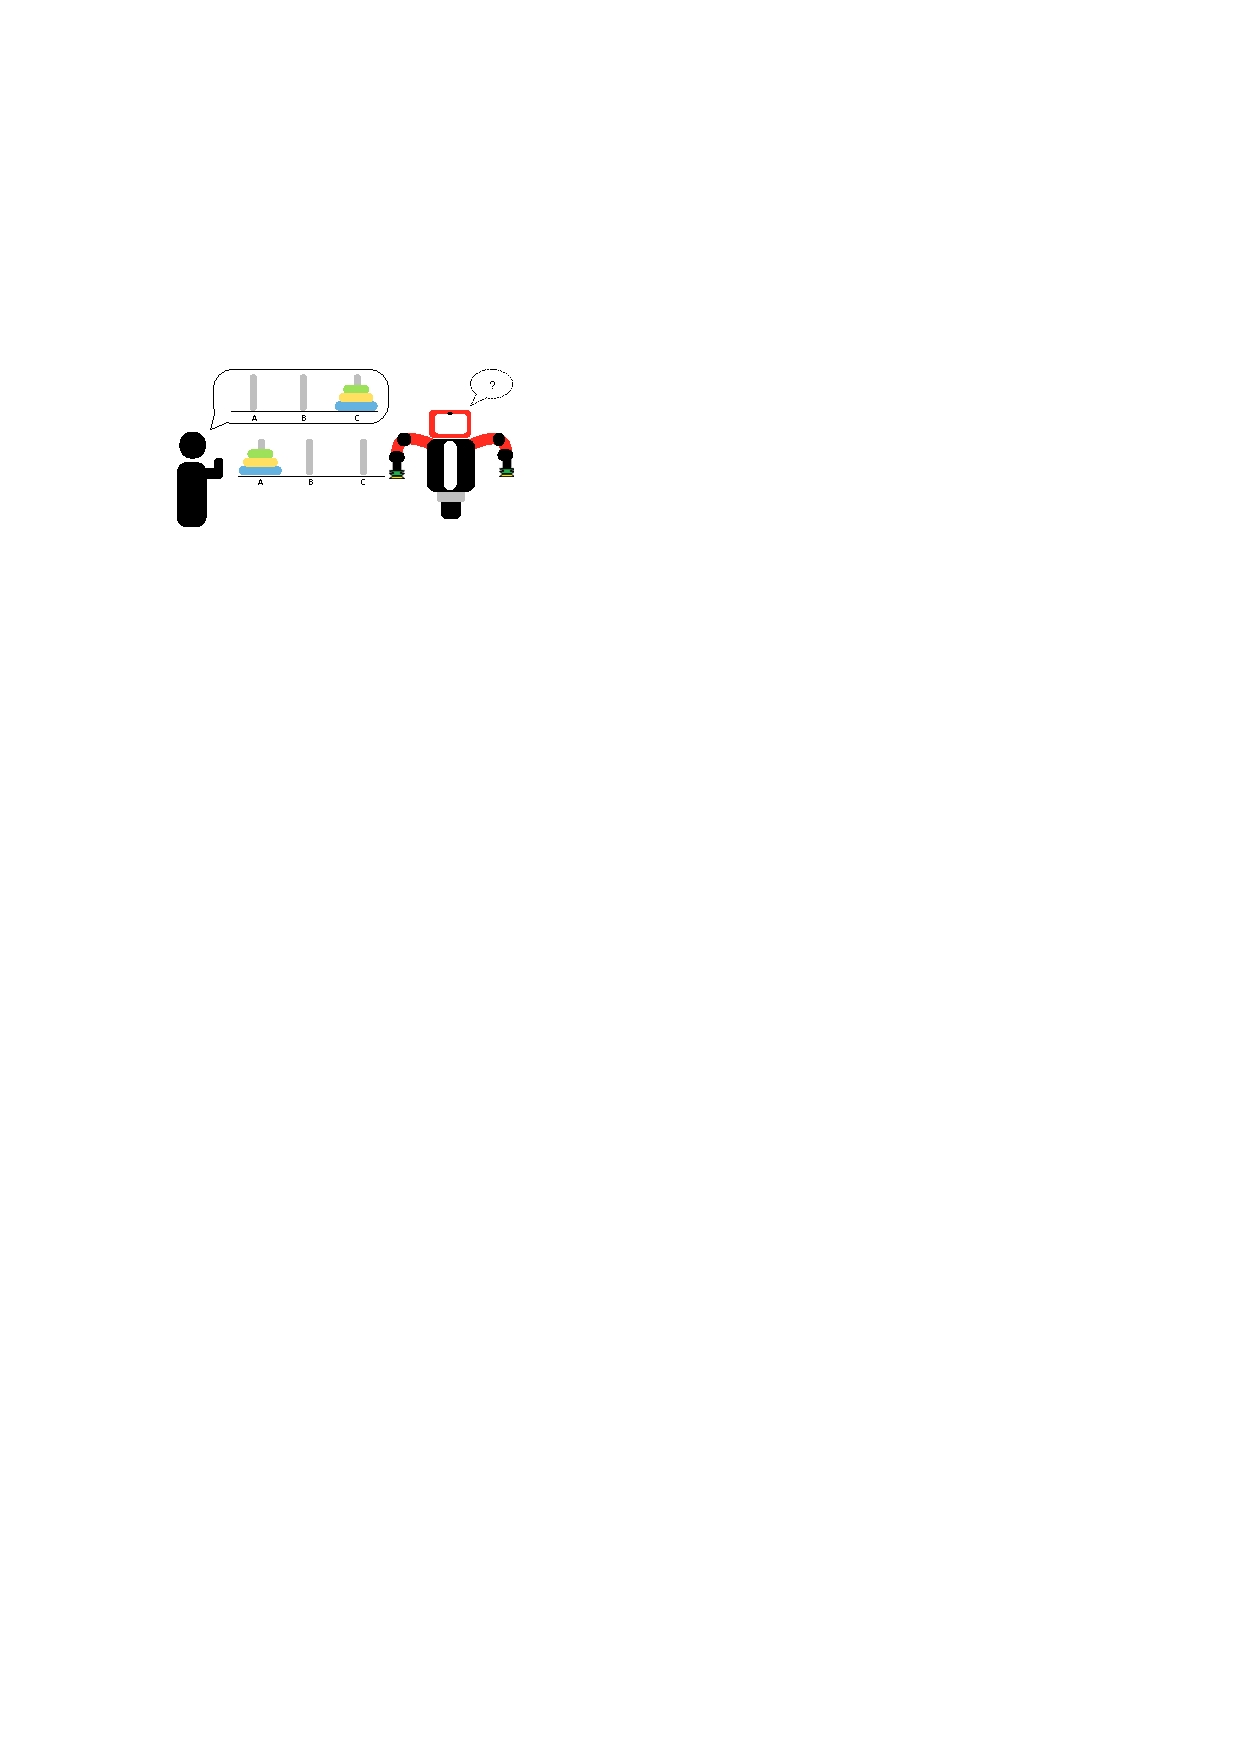
\includegraphics[width=.4\textwidth]{figures/hanoi-0}\hspace{2cm}%\hfill
	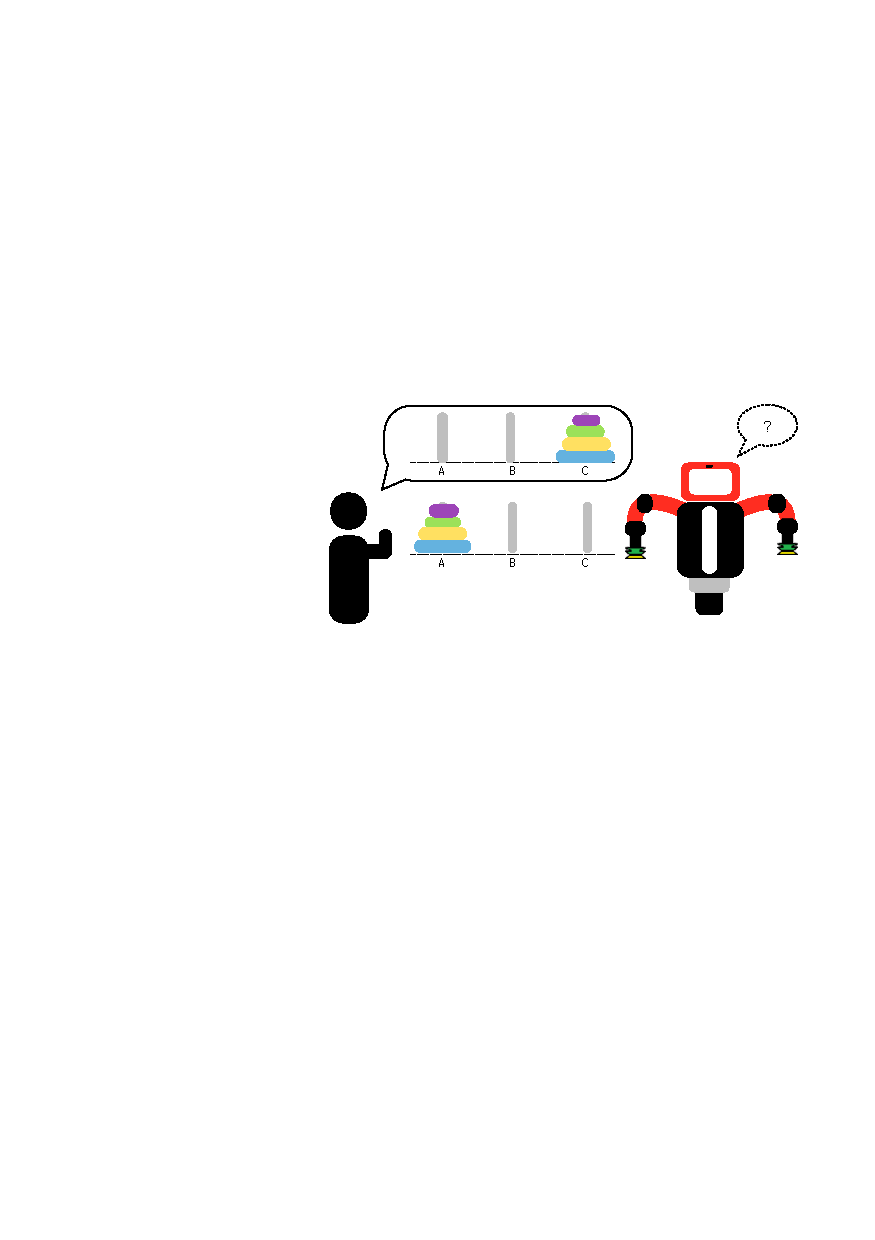
\includegraphics[width=.4\textwidth]{figures/hanoi-1}
	\caption{Tower of Hanoi problem a) with three disks b) with four disks}
	\label{fig:Tower of Hanoi}
\end{figure}

\subsection{Automated Planning}
Automated Planning, also known as \textit{AI Planning}, is a research field that focuses on the development of efficient search algorithms to generate solutions to problems.
Given a set of actions, a description of the state of the world, and some goal state, the planner generates a sequence of actions, which guarantees the transition from the initial state to the goal state (\fig{fig:Planning domain and action}).
To allow a correct transition between different states of the world, actions are defined in terms of preconditions and effects (\fig{fig:Planning domain and action}b). 
Planning algorithms use a symbolic planning language such as STRIPS (\cite{fikes1971strips}) or PDDL (\cite{ghallab2004automated}) as their standard encoding language.
The Tower of Hanoi problem could be defined as a planning problem and solved for any number of disks using an automated planner.
%In the initial state, the disks are stacked in ascending order (smallest at the top) on one of the pegs, in the goal state the disks are stacked in the same order on one of the other two remaining pegs. 
%The goal state must be achieved by obeying certain rules for moving the disks (e.g. only the top disk of a stack can be moved at a time and may not be placed on top of a smaller disk). 


\begin{figure}[htp]
	\centering
	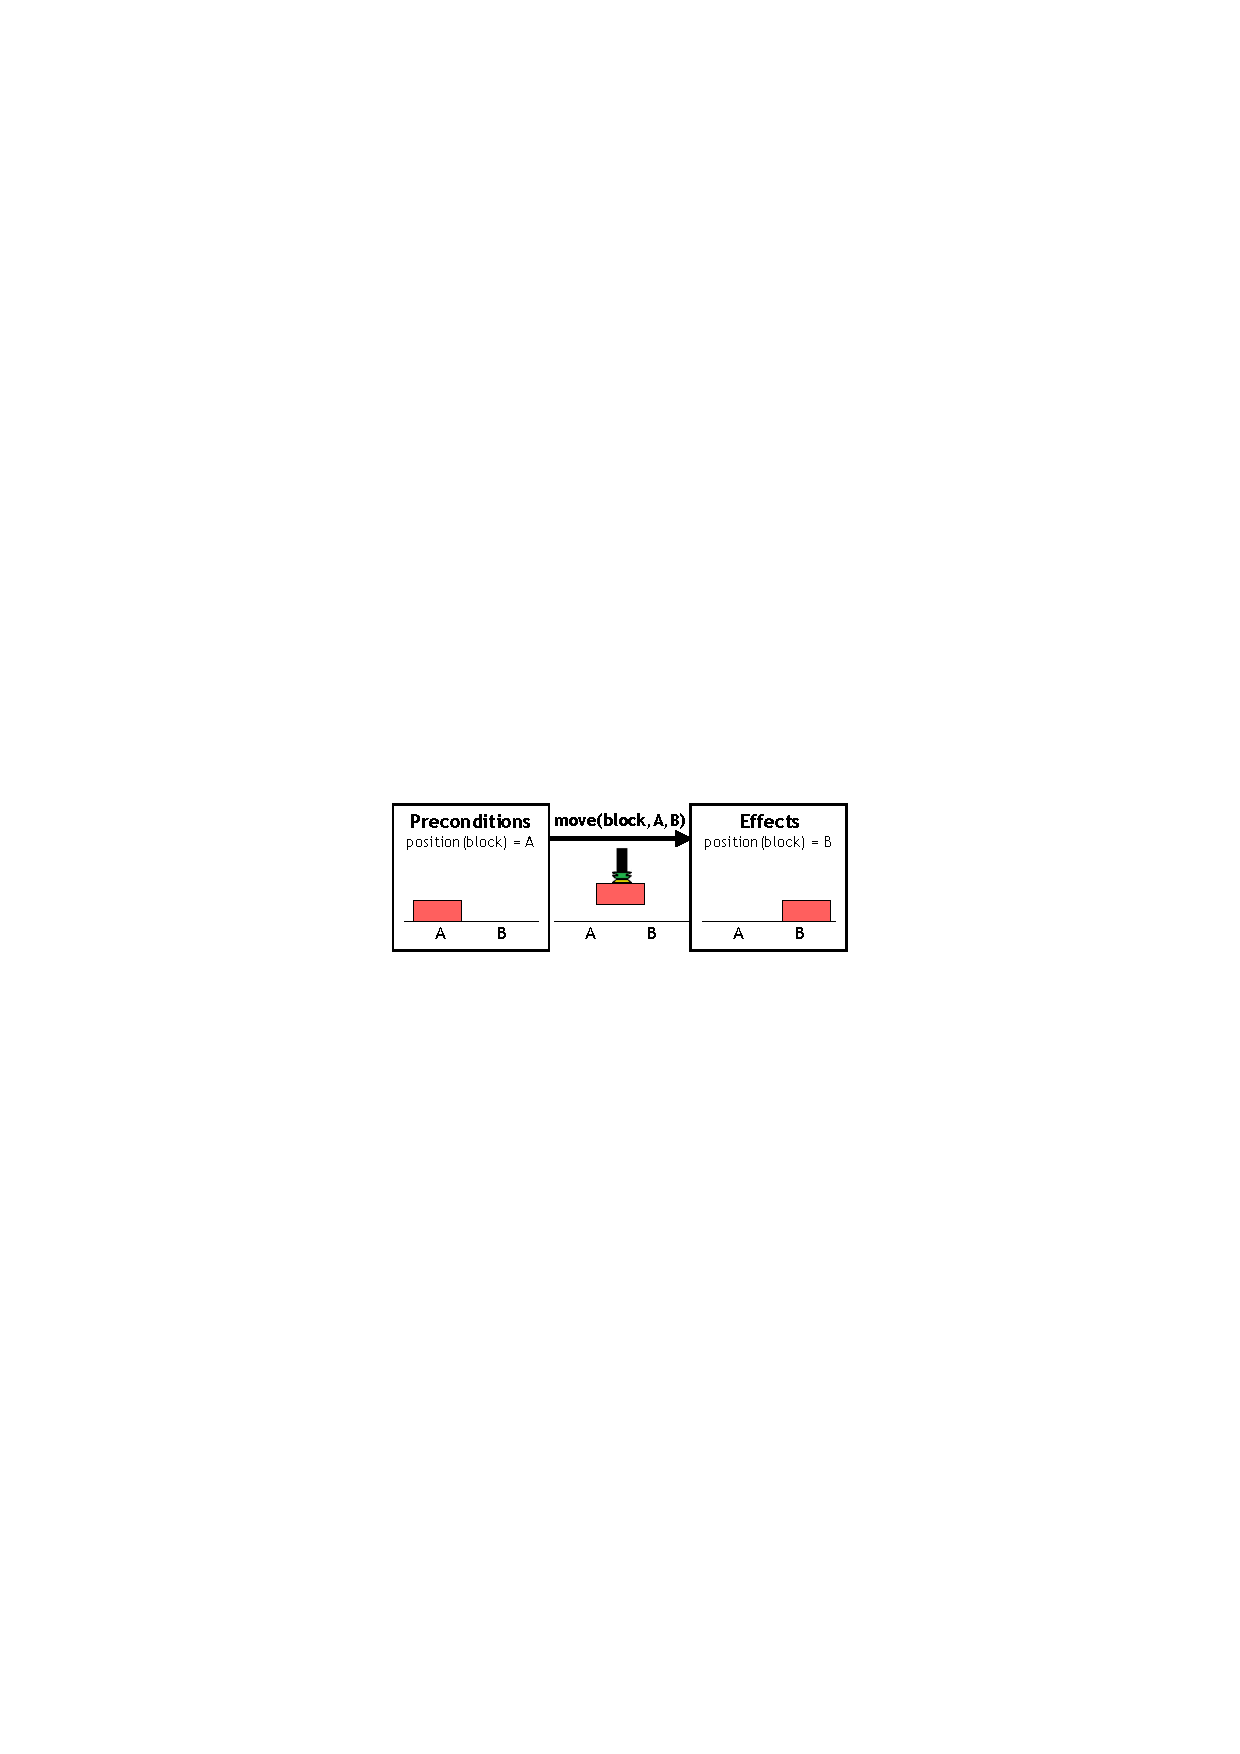
\includegraphics[width=.4\linewidth]{figures/schema-logic-1}
	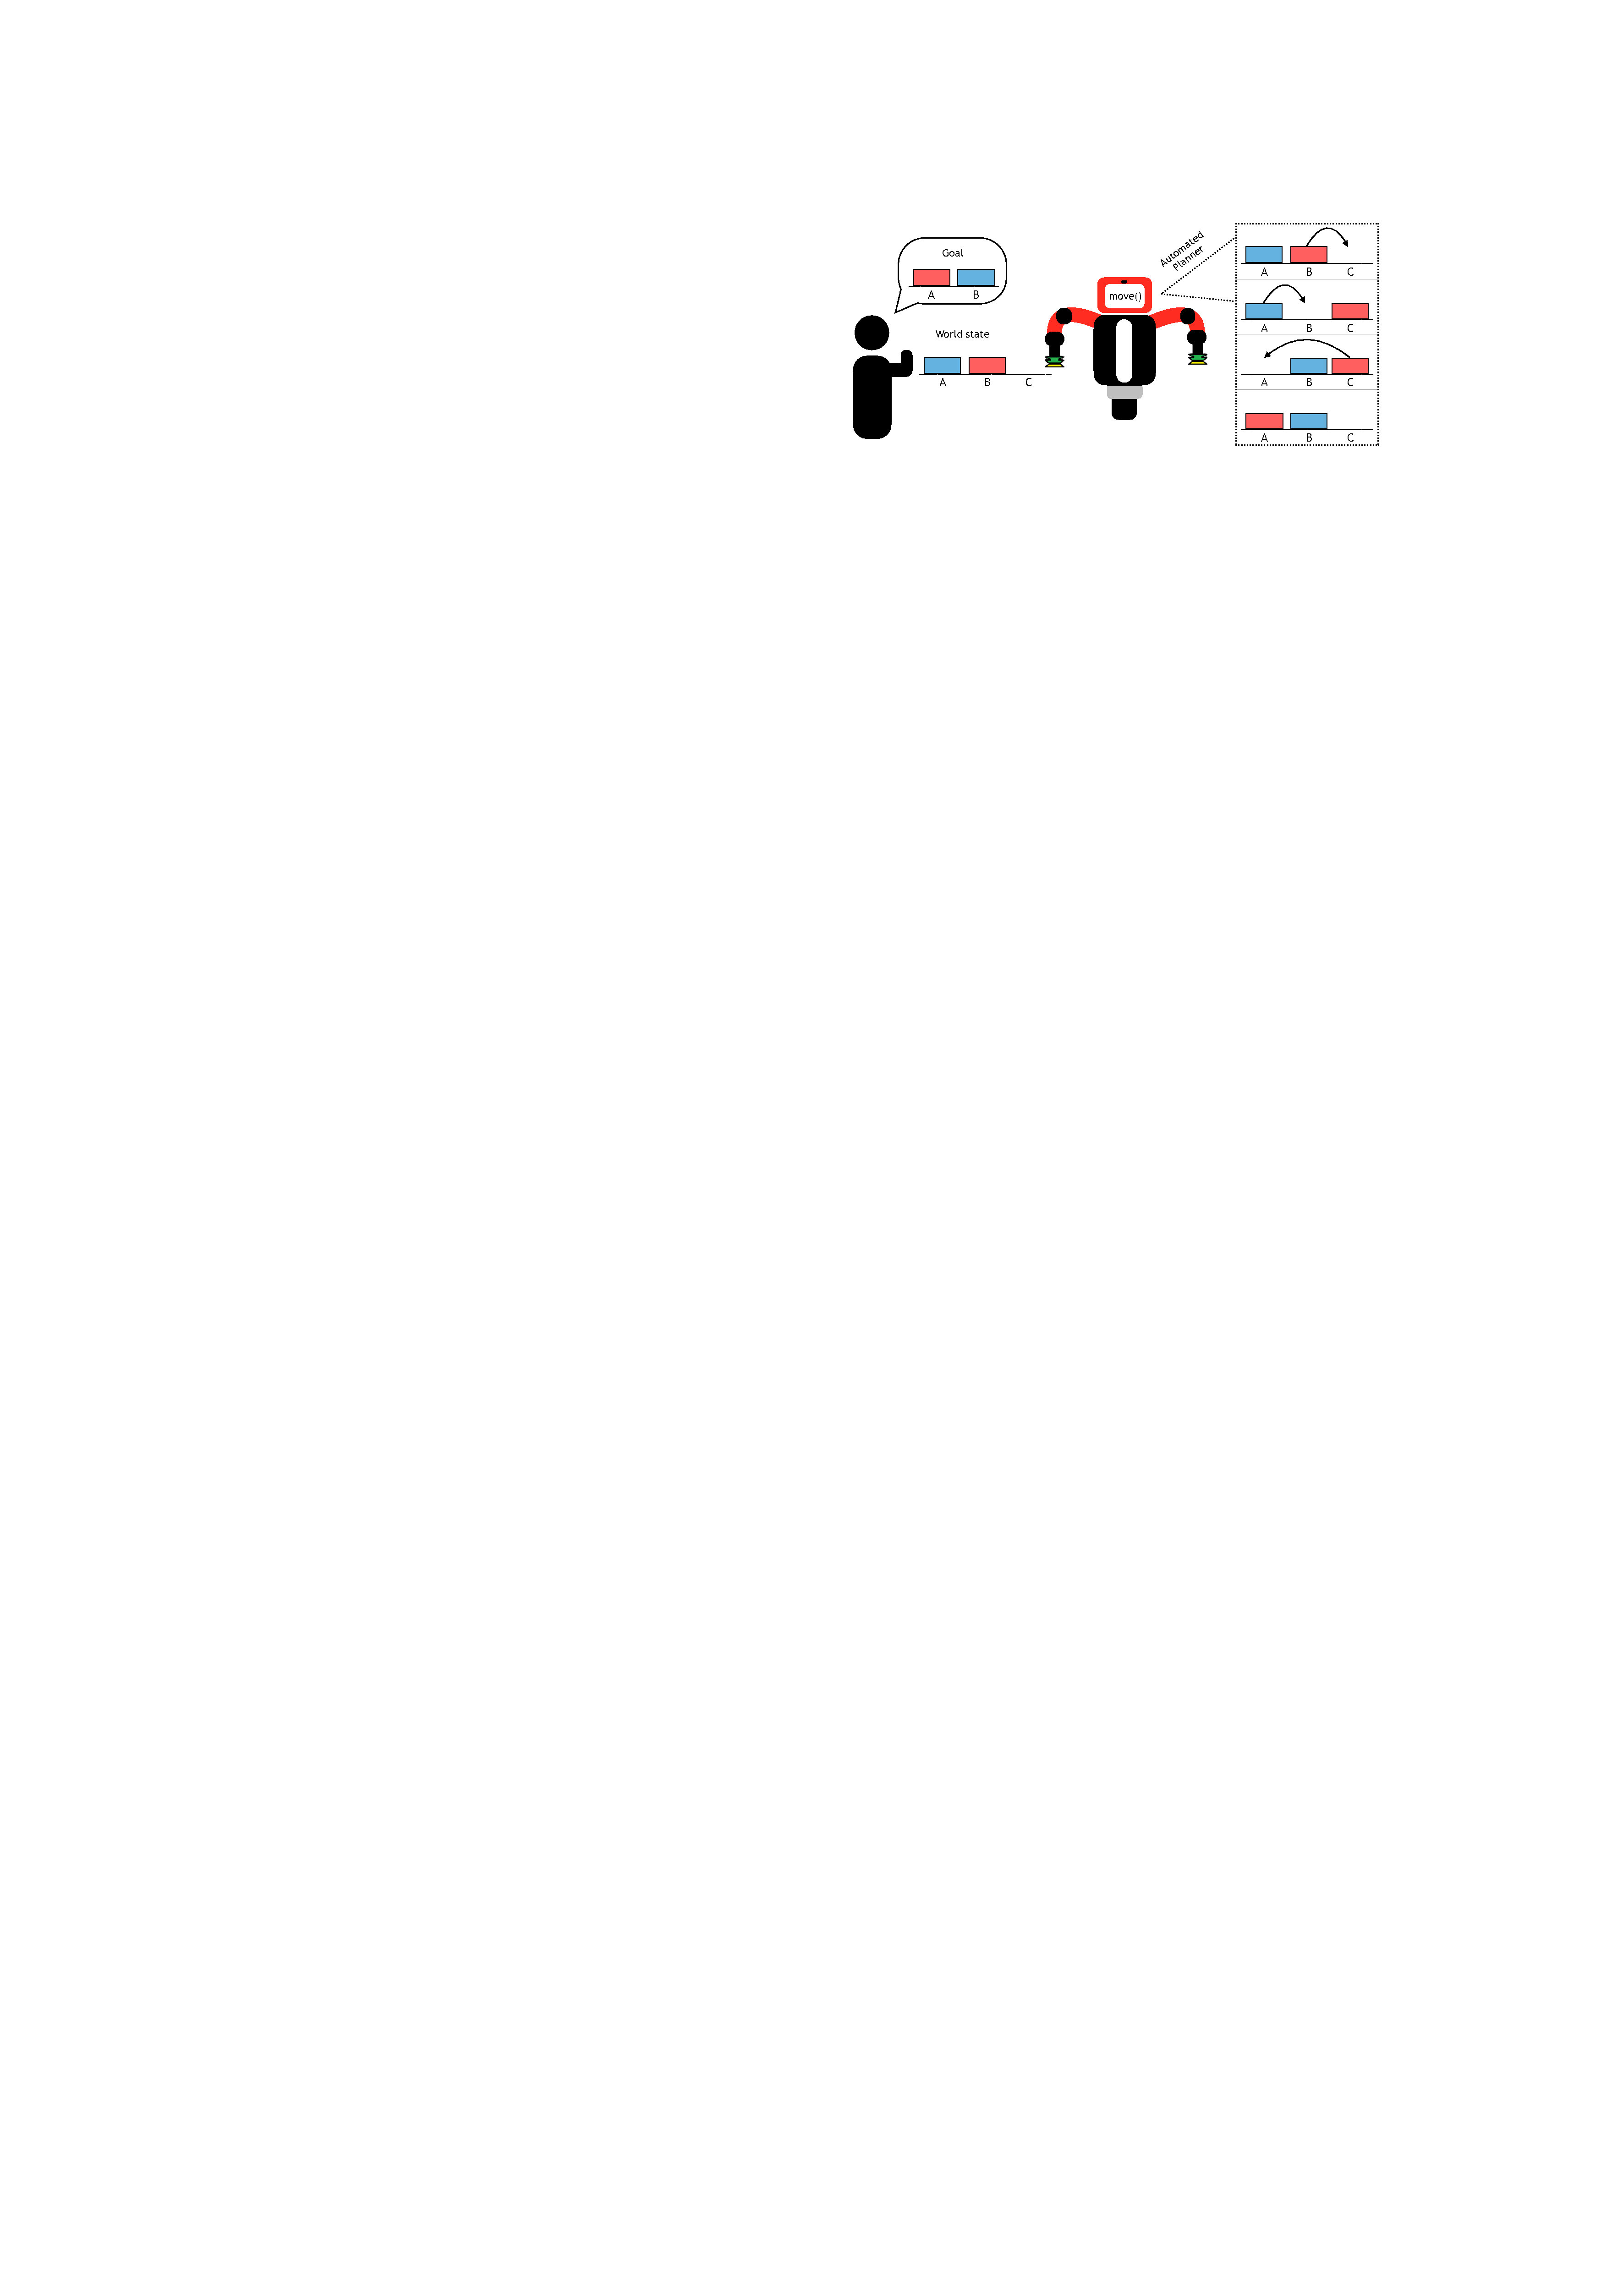
\includegraphics[width=.55\linewidth]{figures/PbD-AutomatedPlanner}
	\caption{Planning domain describing action model with preconditions and effects (left), an initial world state, goal state, and a generated action sequence (right).}
	\label{fig:Planning domain and action}
\end{figure}

% teaching action semantics
Current approaches only teach the robot an action for manipulating an object, but do not explicitly associate a semantic meaning to it, other than assigning it a name.
If the robot is taught an action's semantic meaning, i.e. the conditions for executing the action, it is provided with the relevant application context and could reuse the action in different contexts.
For example, the robot is taught to pick up an object from an initial position and place it on a goal position.
Conditions for executing this action (e.g. to grab an object only if the gripper is free) are generally neglected during the demonstration.
If the teacher demonstrates a pick-up action to the robot, there is no mention of communicating the conditions for when it can execute the action.


\subsection{Problem Statement}
% limitations 
We need to consider the limitations: limited resources, lack of programming knowledge and time to train operators.
%, rather than atomic actions that can be reused independently 

We want the robot to generate solutions autonomously.
For this we need:
Automated planner - which as the robot's \textit{``brain"}
action models - actions with semantic meaning associated to it
PbD - end-user technique to teach robot an action

% semantics for application to new context
A robot that learns how to arrange items on a desk may have to plan the order of handling objects in another way than originally demonstrated by the teacher.
Thus, it does not suffice for the robot to replicate the demonstrated movement, but it needs to understand and interpret the teacher's intention so that it can apply the action to different scenarios.


In this thesis, we propose a framework that allows robots to solve problems in a goal-oriented way.
In other words, given a user-defined goal, the robot should generate and execute the right action sequence to obtain it.
The user must construct a knowledge base, consisting of a domain model (the environment that the robot interacts with) and all action models required for the robot to accomplish the defined task.

% example domain 
Consider again the Tower of Hanoi problem.
The domain model would consist of a table with a finite number of objects and limited positions, as well as actions consisting of pick, place and move. 
Possible goals could be to stack the objects by size (similar to the Tower of Hanoi problem) or to arrange the objects in a certain order. 
Our framework should enable the user to teach the robot by demonstration all action models needed, including their relevant preconditions and effects. 
Once the action models have been created, the inbuilt automated planner can generate an action sequence to achieve any goal within the domain. 

%Hence, we address two common situations, where reprogramming is required: 
%\begin{itemize}
%\item A new subtask needs to be included in the task execution, e.g. the robot knows how to place objects from any position on the table into a basket, but should additionally rotate them before placing them;
%\item All subtasks are available but the ultimate goal has changed, e.g. the order of placing the objects has been changed.
%\end{itemize}

